\documentclass[letterpaper]{article}

\usepackage[letterpaper,margin=1in]{geometry}
\usepackage{xcolor}
\usepackage{tikz}
\usepackage{graphicx}
\usepackage{setspace}
\usepackage{lmodern}
\usepackage{hyperref}

\graphicspath{ {../images/} }
\usepackage[margin=1in]{geometry}
\usepackage{tikz}
\usepackage[dvipsnames]{xcolor}
\usetikzlibrary{calc}


\newcommand{\titleDOC}{Title}
\newcommand{\authorDOC}{Daniel Sabalakov}
\newcommand{\dateDOC}{\today}
\newcommand{\classDOC}{DE Intro to Doodlehickies}
\newcommand{\emailDOC}{danielsabalakov@gmail.com}
% DEFAULT QUOTE IS BY ISSAC NEWTON. IF YOU DON'T WANT IT, DO: quote: @none
\newcommand{\quoteDOC}{``\textit{Truth is ever to be found in the simplicity, and not in the multiplicity and confusion of things}'' - Issac Newton}


\usepackage{graphicx} % Required for inserting images

\begin{document}
\newcounter{none}

% This is a template title page that I will be using for my projects
% Credit where credit is due: I began with this template
% https://www.reddit.com/r/LaTeX/comments/faij1n/my_first_cover_page_done_in_latex_is_it/
\begin{titlepage}



\pagestyle{empty}
% Begin tikz picture, remember the picture
\begin{tikzpicture}[overlay,remember picture]

% Node(s) 1: Death Star
\newcommand{\baseSTARX}{14}
\newcommand{\baseSTARY}{-2}
\newcommand{\baseDISCX}{\baseSTARX - 1}
\newcommand{\baseDISCY}{\baseSTARY - 0.3}
\newcommand{\baseDISCR}{1}

\node[circle, text=white,minimum size=7cm, fill=lightgray] at (\baseSTARX,\baseSTARY) {};
\node[circle, text=white,minimum size=2cm, fill=gray] at (\baseDISCX,\baseDISCY) {};

% Node(s) 2: Alderran
\newcommand{\basePLANETX}{1}
\newcommand{\basePLANETY}{-4}
\node (planet) at (\basePLANETX,\basePLANETY) {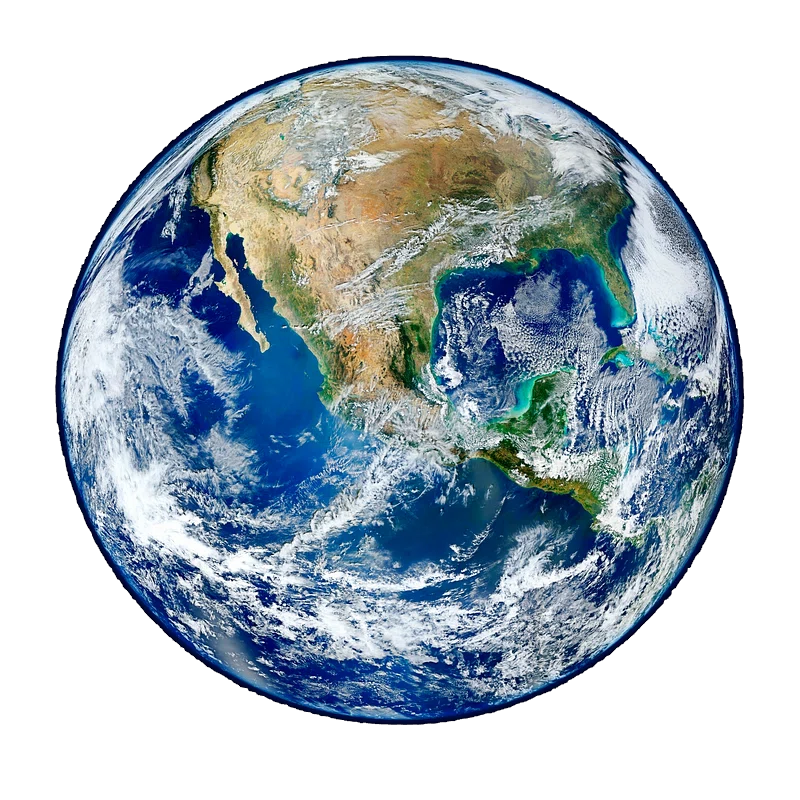
\includegraphics[width=3cm]{earthEDITED.png}};

%Node(s) 3: Laser
\newcommand{\baseFOCIX}{3}
\newcommand{\baseFOCIY}{-3}
%modX
\draw [green, very thick] (\baseFOCIX,\baseFOCIY) -- (\baseDISCX + \baseDISCR,\baseDISCY);
\draw [green, very thick] (\baseFOCIX,\baseFOCIY) -- (\baseDISCX - \baseDISCR,\baseDISCY);

%modY
\draw [green, very thick] (\baseFOCIX,\baseFOCIY) -- (\baseDISCX,\baseDISCY + \baseDISCR);
\draw [green, very thick] (\baseFOCIX,\baseFOCIY) -- (\baseDISCX,\baseDISCY - \baseDISCR);


% END GRAPHICS



% TITLE OF DOCUMENT
\node at ($(current page.center)+(0,2)$) {{\fontsize{60}{72} \selectfont \titleDOC}};
% AUTHOR, CLASS, DATE
\node[text width=8in,align=center] at ($(current page.center)+(0,0)$) {{\fontsize{16}{19.2} \selectfont \textcolor{orange}{ \bf \authorDOC}} \\[6pt] \classDOC\\[6pt] \dateDOC};
% QUOTE
\node[text width=8in,align=center] at ($(current page.center)+(0,-4)$) { \fontsize{16}{19.2} \selectfont \quoteDOC};


% \node[text width=1.1in,align=center] at ($(current page.center)+(8.5,-13)$) {{
%     Generated by Scoresh's Lab-Gen
% }};


\end{tikzpicture}

% \begin{figure}[htbp]
%     \centering
%     
\includegraphics[width=0.3\textwidth]{images/labgenpng.png}
% \end{figure}


\end{titlepage}









\end{document}
